
\documentclass[../main.tex]{subfiles}

\begin{document}


%
% -----------------------------------------------------------------------------------------------------------------
%





%
% -----------------------------------------------------------------------------------------------------------------
%



\begin{frame}[fragile]{Open questions and improvements}

\begin{columns}[c]

\begin{column}{0.8\linewidth}
\begin{itemize}
\item Power systems
\begin{itemize}
\item Extension to the three phases unbalanced case
\item Topology verification tool
\end{itemize}
\item Multi-frequency allocation problem
\begin{itemize}
\item Theoretical guarantees (if possible)
\end{itemize}
\end{itemize}
\end{column}

\begin{column}{0.2\linewidth}
\centering
\includegraphics[scale=0.1]{pics/question_mark.png}
\end{column}
\end{columns}

\end{frame}


\begin{frame}[t, allowframebreaks]
\frametitle{References}
\bibliographystyle{IEEEtran}
\bibliography{Refs}
\end{frame}

\backupbegin

\begin{frame}[t]
\end{frame}

\begin{frame}[t]{Extra. Motivation. Examples}
\begin{itemize}
\item Keep network model updated
\begin{itemize}
\item Cables aging;
\item Connection problems;
\item Undocumented cable changes (after breaks, faults etc.);
\end{itemize}
\end{itemize}
\end{frame}


\begin{frame}[t, noframenumbering]{Extra. Motivation. Examples}
\begin{itemize}
\item Keep network model updated
\begin{itemize}
\item Cables aging;
\item Connection problems;
\item Undocumented cable changes (after breaks, faults etc.);
\end{itemize}
\item Fault prevention and localisation (LV cable faults change from transient to permanent);
\begin{columns}
\begin{column}{0.6\textwidth}
\centering
\begin{figure}[H]
\begin{tikzpicture}
\draw[dotted, thick] (0,0) -- (1,0);
\draw[thick] (1,0) -- node[above, red]{\LARGE $\text{\Lightning}$}(6,0);
\draw[fill] (1,0) circle [radius=0.1] node[above]{$\mathbf{SM}_{n}$};
\draw[arrows = {-Stealth[fill=none, inset=0pt, angle=90:10pt]}, thick] (1,0) -- (1,-2);
%\draw[arrows = {-Stealth[inset=0pt, angle=30:10pt]}, thick] (1,0) -- (1,-1) node[left]{$\mathbf{i}_{n}$};
\draw[fill] (6,0) circle [radius=0.1] node[above]{$\mathbf{SM}_{n+1}$};
\draw[arrows = {-Stealth[fill=none, inset=0pt, angle=90:10pt]}, thick] (6,0) -- (6,-2);
%\draw[arrows = {-Stealth[inset=0pt, angle=30:10pt]}, thick] (6,0) -- (6,-1) node[left]{$\mathbf{i}_{n+1}$};
\draw[dotted, thick] (6,0) -- (7,0);
\end{tikzpicture}
\end{figure}
\end{column}
\begin{column}{0.4\textwidth}
\centering
\begin{figure}[H]
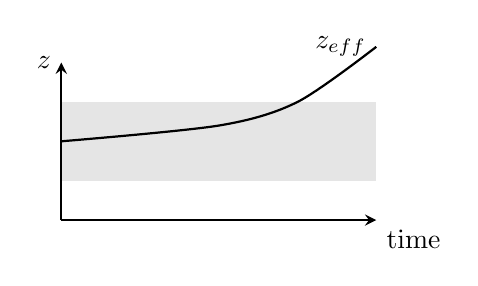
\begin{tikzpicture}
\draw[fill=gray!20, draw opacity=0] (0,0.5) -- (0,1.5) -- (4,1.5) -- (4,0.5) -- cycle;
%\draw[fill=red!20, draw opacity=0] (0,1) -- (2,1.2) -- (2,0) -- (0,0) -- cycle;
%\draw[dashed, fill=gray!20] plot[smooth cycle] coordinates {(0,1) (2,1.2)};
\draw[thick, ->, >=stealth] (0,0) -- (4,0) node[anchor=north west] {time};
%\draw[dashed, fill=gray!20] plot[smooth cycle] coordinates {(0,1) (2,1.2) (2,0) (0,0)};
%\uncover<2->{\draw[thick, dotted] (0,1) -- (4, 1)node[right]{$z_{line}$};}
\draw[thick, black] plot [smooth] coordinates {(0,1) (2,1.2) (3,1.5) (4,2.2)}  node[left] {$z_{eff}$};
\draw[thick, ->, >=stealth] (0,0) -- (0,2) node[left]{$z$};
\end{tikzpicture}
\end{figure}
\end{column}
\end{columns}
\end{itemize}
\end{frame}



\begin{frame}[t, noframenumbering]{Extra. Motivation. Examples}
\begin{itemize}
\item Keep network model updated
\begin{itemize}
\item Cables aging;
\item Connection problems;
\item Undocumented cable changes (after breaks, faults etc.);
\end{itemize}
\item Fault prevention (LV cable faults change from transient to permanent);
\item Stealing detection (hooking):
\begin{columns}
\begin{column}{0.6\textwidth}
\centering
\begin{figure}[H]
\begin{tikzpicture}
\draw[dotted, thick] (0,0) -- (1,0);
\draw[thick] (1,0) -- (6,0);
\draw[fill] (1,0) circle [radius=0.1] node[above]{$\mathbf{V}_{n}$};
%\draw[arrows = {-Stealth[inset=0pt, angle=30:10pt]}, thick, visible on=<1-2>] (1,0) -- (2.5,0)  node[below]{$\mathbf{j}_{n}$};
%\draw[arrows = {-Stealth[inset=0pt, angle=30:10pt]}, thick, visible on=<5->] (1,0) -- (2.5,0)  node[below]{$\mathbf{j}_{n}$};
%\draw[arrows = {-Stealth[inset=0pt, angle=30:10pt]}, thick, visible on=<3-4>] (1,0) -- (2.5,0)  node[below, red]{$\mathbf{j}_{n} + \Delta\mathbf{j}_{n}$};
\draw[arrows = {-Stealth[inset=0pt, angle=30:10pt]}, thick] (1,0) -- (2.5,0)  node[below, red]{$\mathbf{j}_{n} + \Delta\mathbf{j}_{n}$};
\draw[arrows = {-Stealth[fill=none, inset=0pt, angle=90:10pt]}, thick] (1,0) -- (1,-2);
%\draw[arrows = {-Stealth[inset=0pt, angle=30:10pt]}, thick] (1,0) -- (1,-1) node[left]{$\mathbf{i}_{n}$};
%\draw[fill] (6,0) circle [radius=0.1] node[above, visible on=<1-3>]{$\mathbf{V}_{n+1}$};
%\draw[fill] (6,0) circle [radius=0.1] node[above, visible on=<5->]{$\mathbf{V}_{n+1}$};
%\draw[fill] (6,0) circle [radius=0.1] node[above, visible on=<4>]{$\mathbf{V}_{n+1} + \Delta\mathbf{V}_{n+1}$};
\draw[fill] (6,0) circle [radius=0.1] node[above]{$\mathbf{V}_{n+1} + \Delta\mathbf{V}_{n+1}$};

% theft
%\draw[fill, visible on=<2-4>] (3.5,0) circle [radius=0.1] node[above]{Thief};
\draw[fill] (3.5,0) circle [radius=0.1] node[above]{Thief};
%\draw[arrows = {-Stealth[inset=0pt, angle=30:10pt]}, thick, visible on=<4>] (3.5,0) -- (5,0)  node[below, red]{$\mathbf{j}_{n}$};
\draw[arrows = {-Stealth[inset=0pt, angle=30:10pt]}, thick] (3.5,0) -- (5,0)  node[below, red]{$\mathbf{j}_{n}$};
%\draw[arrows = {-Stealth[fill=none, inset=0pt, angle=90:10pt]}, dotted, thick, visible on=<2-4>] (3.5,0) -- (3.5,-2);
\draw[arrows = {-Stealth[fill=none, inset=0pt, angle=90:10pt]}, dotted, thick] (3.5,0) -- (3.5,-2);
%\draw[arrows = {-Stealth[inset=0pt, angle=30:10pt]}, thick, visible on=<4>] (3.5,0) -- (3.5,-1) node[left, red]{$\Delta\mathbf{j}_{n}$};
\draw[arrows = {-Stealth[inset=0pt, angle=30:10pt]}, thick] (3.5,0) -- (3.5,-1) node[left, red]{$\Delta\mathbf{j}_{n}$};

\draw[arrows = {-Stealth[fill=none, inset=0pt, angle=90:10pt]}, thick] (6,0) -- (6,-2);
%\draw[arrows = {-Stealth[inset=0pt, angle=30:10pt]}, thick] (6,0) -- (6,-1) node[left]{$\mathbf{i}_{n+1}$};
\draw[dotted, thick] (6,0) -- (7,0);
\end{tikzpicture}
\end{figure}
\end{column}
\begin{column}{0.4\textwidth}
\centering
\begin{figure}[H]
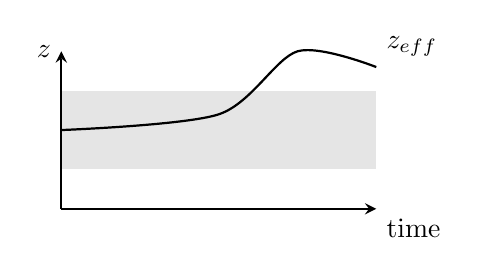
\begin{tikzpicture}
\draw[fill=gray!20, draw opacity=0] (0,0.5) -- (0,1.5) -- (4,1.5) -- (4,0.5) -- cycle;
\draw[thick,->, >=stealth] (0,0) -- (4,0) node[anchor=north west] {time};
%\draw[black, thick] plot [smooth] coordinates {(0,1) (2,1.2) (3,2) (4,1.2)};
% \draw[black, thick, visible on=<1-3>] plot [smooth] coordinates {(0,1) (2,1.2)} node[above left]{$z_{eff}$};
% \draw[black, thick, visible on=<4>] plot [smooth] coordinates {(0,1) (2,1.2) (3,2)} node[left]{$z_{eff}$};
% \draw[black, thick, visible on=<5->] plot [smooth] coordinates {(0,1) (2,1.2) (3,2) (4,1.2)} node[above right]{$z_{eff}$};
\draw[black, thick] plot [smooth] coordinates {(0,1) (2,1.2) (3,2) (4,1.8)} node[above right]{$z_{eff}$};
%\uncover<6->{\draw[thick, dotted] (0,1) -- (4, 1)node[right]{$z_{line}$};}
\draw[thick,->, >=stealth] (0,0) -- (0,2) node[left]{$z$};
\end{tikzpicture}
\end{figure}
\end{column}
\end{columns}
\end{itemize}
\end{frame}



\begin{frame}[t, noframenumbering]{Extra. Motivation. Examples}
\begin{itemize}
\item Topology identification (error correction):
\begin{itemize}
\item Validation tool (hypothesis testing);
\item Combination with topology identification approaches.
\end{itemize}
\end{itemize}
\begin{columns}[t]
\begin{column}{0.6\textwidth}
\centering
\begin{figure}[H]
\begin{tikzpicture}
\draw[thick, visible on=<6->] (2,0) -- (8,0);
\draw[thick, visible on=<6->] (6,0) -- (6,-2) -- (8,-2);
\draw[thick, visible on=<6->] (2,0) -- (2,-2) -- (2,-4);
\draw[thick, dotted, visible on=<4-4>] (8,-2) -- node[above]{\textbf{?}}(6,-2);
\draw[thick, visible on=<5-5>] (8,-2) -- node[above, green]{\CheckmarkBold}(6,-2);
\draw[thick, dotted, visible on=<2-2>] (8,-2) -- node[left]{\textbf{?}} (8,0);
\draw[thick, dotted, visible on=<3-3>] (8,-2) -- node[left, red]{\textbf{x}} (8,0);
\draw[fill] (2,0) circle [radius=0.1];
\draw[fill] (4,0) circle [radius=0.1];
\draw[fill] (6,0) circle [radius=0.1];
\draw[fill] (8,0) circle [radius=0.1];
\draw[fill] (6,-2) circle [radius=0.1];
\draw[fill] (8,-2) circle [radius=0.1];
\draw[fill] (2,0) circle [radius=0.1];
\draw[fill] (2,-2) circle [radius=0.1];
\draw[fill] (2,-4) circle [radius=0.1];
\end{tikzpicture}
\end{figure}
\end{column}
\begin{column}{0.4\textwidth}
\centering
\begin{figure}[H]
\begin{tikzpicture}
\draw[fill=gray!20, draw opacity=0] (0,0.5) -- (0,1.5) -- (4,1.5) -- (4,0.5) -- cycle;
\draw[thick, ->, >=stealth] (0,0) -- (4,0) node[anchor=north west] {time};

\draw[thick, black, visible on=<3-3>] plot [smooth] coordinates {(0,1) (1,-1) (2,1.3) (2.5, 0.5) (3, 1.5) (4,-1)};
%\draw[thick, visible on=<3-3>] (0,0) -- (1,-1);
%\draw[thick, visible on=<3-3>] (1,-1) -- (2,2);
%\draw[thick, visible on=<3-3>] (2,2) -- (3,-1);


\draw[thick, black, visible on=<5-5>] plot [smooth] coordinates {(0,1) (1,1.2) (2,1.1) (2.5, 0.9) (3, 1.1) (4,1)};
%\draw[thick, visible on=<5-5>] (0,1) -- (4,1);

%\draw[thick] (0,1) -- (2,1);
%\draw[thick] (2,1) -- (2,2);
%\draw[thick] (2,2) -- (4,2);

\draw[thick, ->, >=stealth] (0,0) -- (0,2) node[anchor=south east] {$z_{eff}$};
\end{tikzpicture}
\end{figure}
\end{column}
\end{columns}
\end{frame}


\begin{frame}[t]{Extra. Related works in impedance identification}
\begin{itemize}
\item Estimation of the Thevenin equivalent grid impedance
\begin{itemize}
\item Many approaches: passive, active, their combinations, etc.
\item High accuracy and good performance
\item Limited applicability. Not suitable for:
\begin{itemize}
\item Fault localisation
\item Detection
\end{itemize}
\end{itemize}
\end{itemize}

\begin{figure}[H]
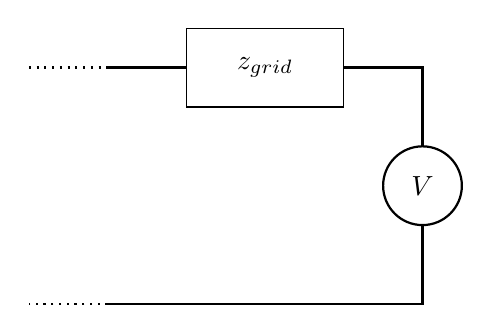
\begin{tikzpicture}
\draw[dotted, thick] (0,0) -- (1,0);
\draw[thick] (1,0) -- (2,0);
\draw (2, -0.5) rectangle node[]{$z_{grid}$} (4, 0.5);
\draw[thick] (4,0) -- (5,0) -- (5, -1);
\draw[thick] (5, -1.5) circle [radius=0.5] node[]{$V$};
\draw[thick] (5,-2) -- (5,-3) -- (1, -3);
\draw[dotted, thick] (1, -3) -- (0, -3);
\end{tikzpicture}
\end{figure}

\end{frame}



\begin{frame}[t, noframenumbering]{Extra. Related works in impedance identification}
\begin{itemize}
\item Estimation of the Thevenin equivalent grid impedance
\item Estimation of the impedance matrix
\begin{itemize}
\item Synchronised (PMU \footnote{Phasor Measurement Unit}, $\mu$PMU) measurements assumption:

\only<2-3>{

\hfill

\hfill

\begin{figure}[H]
\centering
  \begin{tikzpicture}
    \coordinate (t0) at (0, 0.5);
    \coordinate (tn) at (8, 0.5);
    \draw[arrows = {-Stealth[inset=0pt, angle=25:5pt]}] (t0) -- (tn) node[above]{$t$};

    % arrows 1
    \coordinate (a1) at (0, 2);
    \coordinate (c1) at (1.9, 1.7);
    \draw[arrows = {-Stealth[inset=0pt, angle=25:5pt]}] (a1) -- (c1);
    \draw[thin, dotted](a1) -- (0, 0.5);

    \coordinate (a2) at (0,1.5);
    \coordinate (c2_) at (1.9, 1.2);
    \coordinate (c2) at (1.9, 1);
    %\draw[dotted, thin, fill=gray!50] (a2)--(c2)--(c2_)--(a2);
    \draw[arrows = {-Stealth[inset=0pt, angle=25:5pt]}] (a2) -- (c2_);

    \coordinate (text1) at (1, 0);
    \node[text width=2cm] at (text1){time: \cmark \\ phase: \cmark};

    % arrows 2
    \coordinate (a3) at (3,2);
    \coordinate (c3) at (4.9,1.7);
    \draw[arrows = {-Stealth[inset=0pt, angle=25:5pt]}] (a3) -- (c3);
    \draw[thin, dotted](a3) -- (3, 1.5);

    \coordinate (a4) at (3, 1.5);
    \coordinate (a4_) at (3.2, 1.5);
    \coordinate (c4) at (5.1, 1.2);
    \draw[dotted, thin, fill=gray!50] (a4_)--(a4)--(3, 0.5)--(3.2, 0.5)--(a4_);
    \draw[arrows = {-Stealth[inset=0pt, angle=25:5pt]}] (a4_) -- (c4);

    \coordinate (text2) at (4, 0);
    \node[text width=2cm] at (text2){time: \xmark \\ phase: \cmark};

    % arrows 3
    \coordinate (a5) at (6,2);
    \coordinate (c5) at (7.9,1.7);
    \draw[arrows = {-Stealth[inset=0pt, angle=25:5pt]}] (a5) -- (c5);
    \draw[thin, dotted](a5) -- (6, 0.5);

    \coordinate (a6) at (6,1.5);
    \coordinate (c6_) at (7.9, 1.2);
    \coordinate (c6) at (7.9, 1);
    \draw[dotted, thin, fill=gray!50] (a6)--(c6)--(c6_)--(a6);
    \draw[arrows = {-Stealth[inset=0pt, angle=25:5pt]}] (a6) -- (c6);

    \coordinate (text3) at (7, 0);
    \node[text width=2cm] at (text3){time: \cmark \\ phase: \xmark};
  \end{tikzpicture}
\end{figure}
}
\only<3>{
  \begin{itemize}
    \item PMU: time and phased synchronised measurements
    \item \textbf{Proposed approach}: time synchronism only, phases are estimated during computations
  \end{itemize}
}
\end{itemize}
\end{itemize}
\end{frame}

\begin{frame}[t]{Extra}

Consider the following optimisation problem:
\begin{equation}
\begin{aligned}
& \min_{\bm{x}, \bm{y}} 
& & f(\bm{x}, \bm{y}) \\
& \st
& & \bm{y} = \bm{g}(\bm{x}).
\end{aligned}
\label{min_f_xy}
\end{equation}
where:
$f(\bm{x}, \bm{y}) = \|\bm{A}\bm{x} - \bm{B}\bm{y} - \bm{c} \|_2^2$ with $\bm{A} \in \mathbb{R}^{m\times n}$, $\bm{B} \in \mathbb{R}^{m\times n}$, $\bm{c} \in \mathbb{R}^{m}$ and $\bm{g}(\bm{x})$ is a continuous and differentiable function. Introduce $\bm{h}(\bm{y}) \coloneqq \argmin_{\bm{x}} f(\bm{x}, \bm{y})$

\setbeamercolor{block title}{use=structure,fg=black,bg=gray!20}
\begin{lemma}
\label{lemma1}
Assume:
\begin{enumerate}[\color{black}(1)]
\item $\bm{A}$ and $\bm{B}$ are full rank matrices;
\item $\bm{g} \colon \mathbb{R}^m \rightarrow \mathbb{R}^m$ is surjective (onto) mapping; 
\end{enumerate}
Then $\bm{y}^* = \bm{g} \circ \bm{h}(\bm{y}^*)$ and $\bm{x}^* = \bm{h}(\bm{y}^*)$ give the solution $(\bm{x}^*, \bm{y}^*)$ of the optimisation problem (\ref{min_f_xy}).
\end{lemma}

\end{frame}

\begin{frame}[t]{Extra. Illustrative example}

\begin{columns}[T]
\begin{column}{0.35\linewidth}
Given $a, b, c$.

\hfill

$\min_x \|a\sin{x} - bx - c\|_2^2$

\begin{itemize}
\item Objective function value: $1.776...e-15$
\item $x_{min} = -2.27...$
\end{itemize}

\end{column}

\begin{column}{0.65\linewidth}
\includestandalone[scale = 1]{pics/illustrative_example0}
\end{column}
\end{columns}

\end{frame}

\begin{frame}[t]{Extra. Vivaldi antenna}
\begin{figure}[H]
\begin{adjustbox}{width=0.65\linewidth}
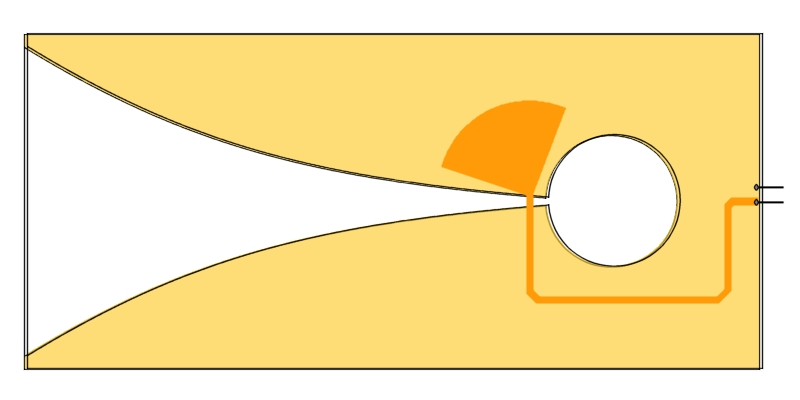
\includegraphics{pics/vivaldi-print.jpg}
\end{adjustbox}
\end{figure}
\end{frame}

\begin{frame}[t]{Extra}
\end{frame}

\begin{frame}[t]{Extra}
\end{frame}
\backupend

\end{document}

